\documentclass{icsc}

\usepackage{booktabs}  % nice tables
\usepackage{siunitx}  % use for all units
\usepackage[margin=2mm]{subcaption}  % for subfigures

\def\kph{\kilo\meter\per\hour}

\pagestyle{empty}

\begin{document}

\begin{center}
  \fontsize{14}{20}{\bf Balance Assist Bicycle Reduces Undesired Motions and\\
  Fall Probability When Subjected to Disturbances\\[3pt]}
\end{center}

%%%%%%%%%%%%%%%% authors %%%%%%%%%%%%%%%
\begin{center}
  \normalsize{\bf{J.~K.~Moore,
                  M.~T.~Haitjema,
                  L.~Alizadehsaravi}}
\end{center}

\begin{center}
  \begin{tabular}{c}
    Faculty of Mechanical Engineering\\
    Delft University of Technology\\
    Mekelweg 2, 2628CD Delft, The Netherlands\\
    e-mail: j.k.moore@tudelft.nl\\
  \end{tabular}
\end{center}

\begin{keywords}
  assist,
  balance,
  bicycle,
  control,
  disturbance,
  fall,
  perturbation
\end{keywords}

\section{INTRODUCTION}
%
The lack of bicycle self-stability at speeds below normal cruising speeds
contribute to falls due the need for acute rider balance control. We have
developed a balance assisting bicycle that uses a custom electric motor to
apply a steering torque in parallel with the rider's steering actions. The
motor is controlled by a simple control algorithm based on feedback from a rate
gyroscope that measures vehicle roll angular rate. Applying a steering torque
in the same direction and proportional to the rolling rate can lower the speed
range at which the bicycle feels self-stable to the rider. We hypothesize that
making the bicycle stable at lower speeds will reduce the control action needed
from the rider in basic balancing tasks and that use of such a system may
reduce falls. We have developed three comprehensive experiments to assess the
effectiveness of the balance assist effects. In the first experiment, we both
distract the rider and apply small disturbances via the steering motor during
straight line balancing. In the second experiment, we apply increasingly large
perturbations to the handlebars via computer controlled ropes while riding on a
treadmill at low speeds. In the final experiment, we perturb straight line
riding via a kickplate, which slides the ground out from under the front wheel
of the bicycle, to see differences in the recovery response with and without
balance assist enabled.

\section{METHODS}
%
To design the controller, we utilized the linear Carvallo-Whipple bicycle model
from \cite{Meijaard2007}. The states are the roll angle \(\phi\) and steer
angle \(\delta\) along with their time derivatives and the inputs are roll
torque \(T_\phi\) and steer torque \(T_\delta\). The state \(\mathbf{A}\) and
input \(\mathbf{B} = \begin{bmatrix}\mathbf{B}_\phi \quad
\mathbf{B}_\delta\end{bmatrix} \) matrices are functions of the equilibrium
forward speed \(v\). The applied steering torque \(T_\delta\) is the sum of the
(h)uman and (m)otor torques, with the motor torque following a proportional
roll rate feedback law scheduled by speed, similar to that shown in
\cite{Schwab2008}:
%
\begin{align}
  T_\delta =
  T_\delta^\textrm{h} + T_\delta^\textrm{m} =
  T_\delta^\textrm{h} - k_{\dot{\phi}}(v - v_\textrm{weave})\dot{\phi}
\end{align}
where \(v_\textrm{weave}\) is the bicycle's open loop weave critical speed.
This gives the closed loop model with the automatic control:
%
\begin{align}
  \begin{bmatrix}
    \dot{\phi} \\ \ddot{\phi} \\ \dot{\delta} \\ \ddot{\delta}
  \end{bmatrix}
  =
  \left(
    \mathbf{A} - \mathbf{B}_\delta
    \left[0 \quad k_{\dot{\phi}}(v - v_\textrm{weave}) \quad 0 \quad 0\right]
  \right)
  \begin{bmatrix}
    \phi \\ \dot{\phi} \\ \delta \\ \dot{\delta}
  \end{bmatrix}
  +
  \mathbf{B}
  \begin{bmatrix} T_{\phi} \\ T_\delta^\textrm{h} \end{bmatrix}
  \textrm{.}
  \label{eq:state-space}
\end{align}

The gain \(k_{\dot{\phi}}\) can be selected such that the eigenvalues of
Equation~(\ref{eq:state-space}) have negative real parts for a range of low
riding speeds, making the bicycle stable.

We developed a series of three experiments, Figure~\ref{fig:experiments}, to
assess whether stabilizing the bicycle is beneficial in safety critical
scenarios:
\begin{description}
  \item[Experiment 1 (E1)] Comparison of 18 older and 14 younger adults in
    straight riding when 1)~looking over their shoulder and 2)~subjected
    to steer motor induced perturbations with assist on and off. We measured
    the standard deviation of steer and roll motions post disturbances.
  \item[Experiment 2 (E2)] Twenty-six young adults were subjected to externally
    applied and measured handlebar torques of varying magnitudes while riding
    on a treadmill at speeds of \qtyrange{6}{10}{\kph}. We determined the
    magnitude of perturbation required to cause them to fall with the balance
    assist system on and off. We logged the order of perturbations and applied
    impulse as well as the bicycle state at the time of perturbation.
  \item[Experiment 3 (E3)] We subjected 11 participants riding at 12~\si{\kph}
    to lateral pulse-like perturbations at the front tire contact patch as they
    rode over a kickplate. We measured the standard deviation of the steer,
    yaw, and roll motions post disturbance with assist on and off.
\end{description}

\begin{figure}[h]
  \begin{center}
    \subcaptionbox{E1: Course layout (left) and GNSS traces
    (right).}{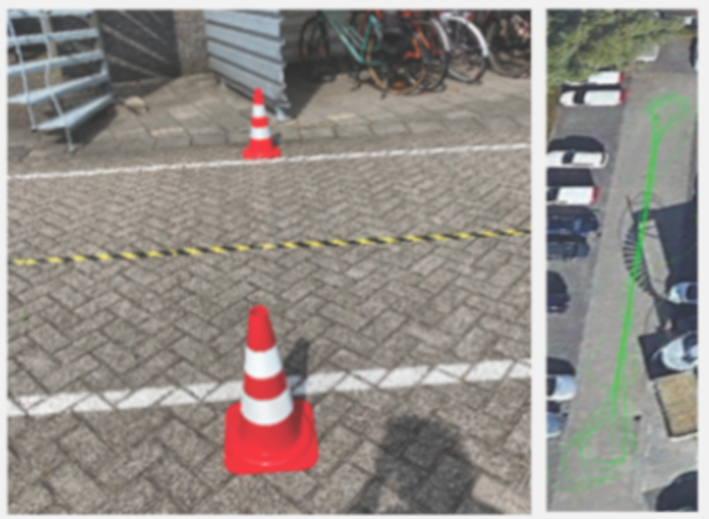
\includegraphics[width=50mm]{old-young-disturbance-experiments.png}}
    \subcaptionbox{E2: During (left) and after (right) handlebar
    perturbation.}{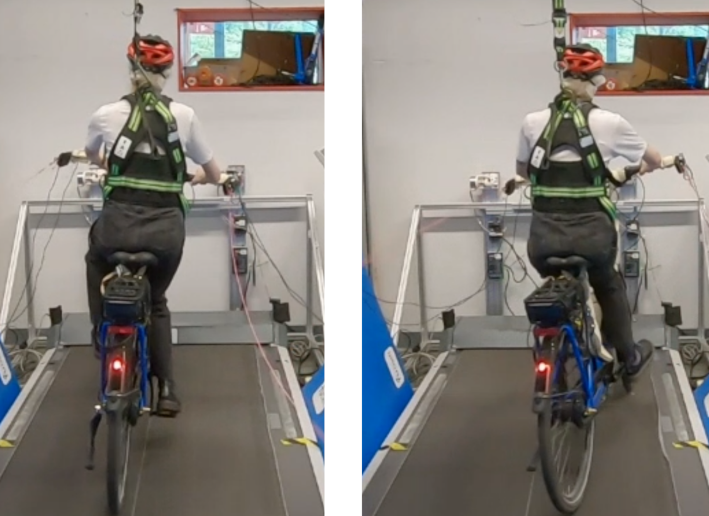
\includegraphics[width=50mm]{perturbation-threshold-experiment.png}}
    \subcaptionbox{E3: Just after leftward front wheel
    kick.}{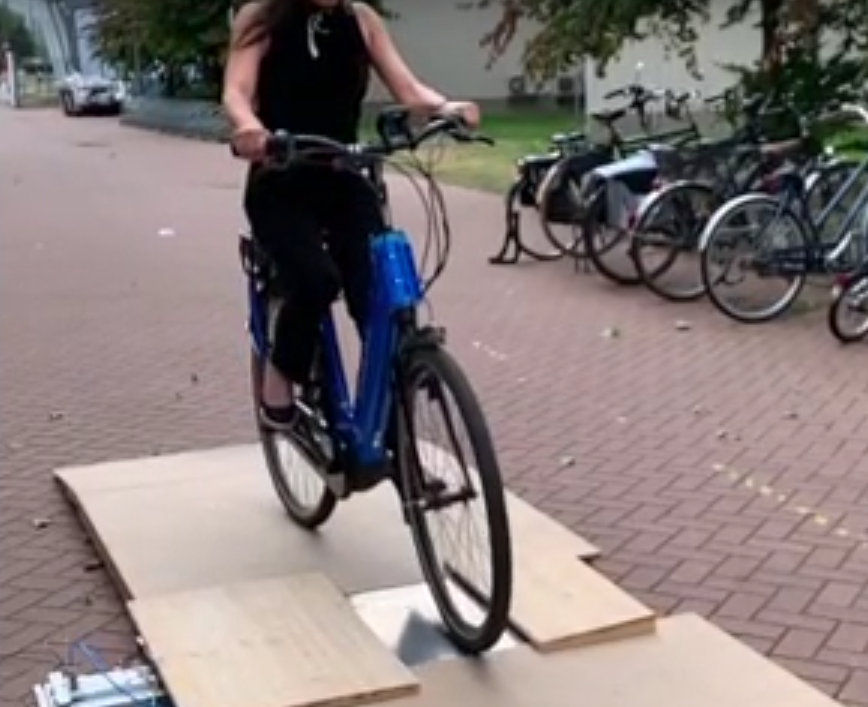
\includegraphics[width=45mm]{kickplate-experiment.png}}
    \caption{Representative images from each experiment.}
    \label{fig:experiments}
  \end{center}
\end{figure}

We then apply multivariate linear regression to the performance metrics derived
from each experiment (ANOVA in E1 \& E3 and logistic in E2) and investigated
whether the balance assist system reduces response motions (E1 \& E3) or the
probability of falling (E2).

\section{Results}
%
In E1, we found that the standard deviation of the roll rate during straight
riding is reduced when the balance assist system is turned on for both young
and old participants. In E2, the probability of falling is significantly
reduced while riding at 6~\si{\kph} when the balance assist system is on. There
is also a reduction in probability at 10~\si{\kph}, but the effect was not
statistically significant (\(p=0.7\)). In Experiment 3, we found that the
standard deviation of steer angle, roll angle, and yaw angle are all
significantly reduced post perturbation when the balance assist system is on.

\begin{figure}[t]
  \begin{center}
    \subcaptionbox{E1 Results: Roll rate standard deviation reduction. Stars
    indicate significant
    difference.}{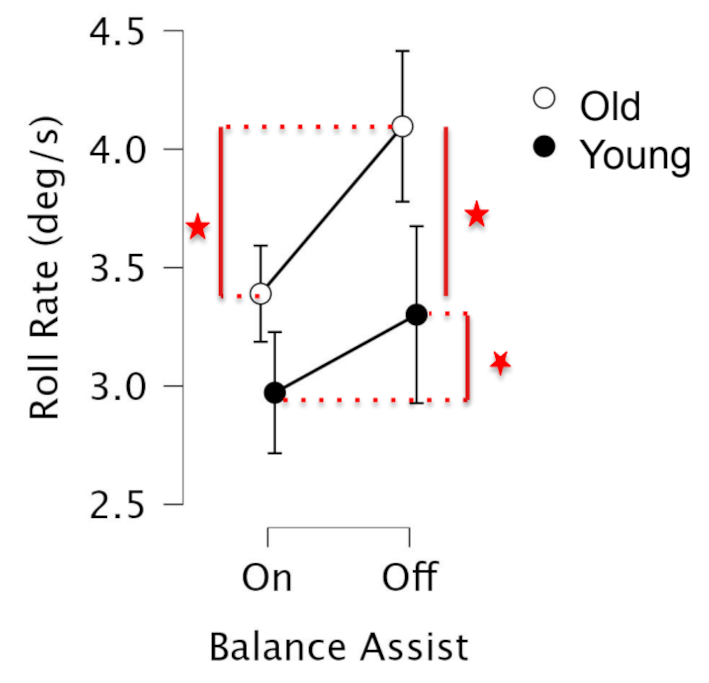
\includegraphics[width=50mm]{old-young-disturbance-results.png}}
    \subcaptionbox{E2 Results: Fall probability as a function of mean centered
    and normalized perturbation
    impulse.}{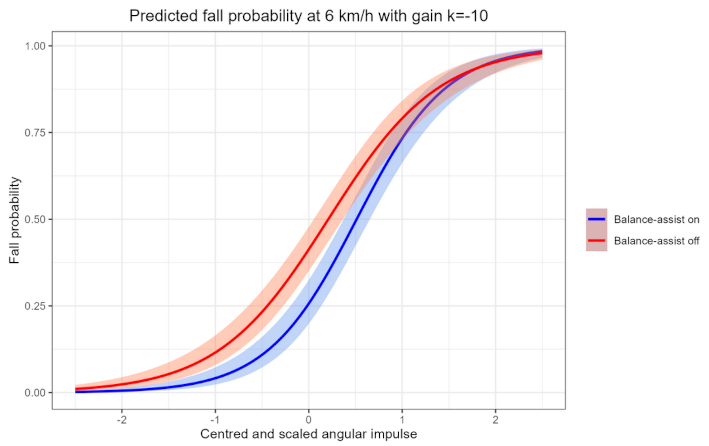
\includegraphics[width=75mm]{perturbation-threshold-results.png}}
    \subcaptionbox{E3 Results: Yaw angle standard deviation
    reduction.}{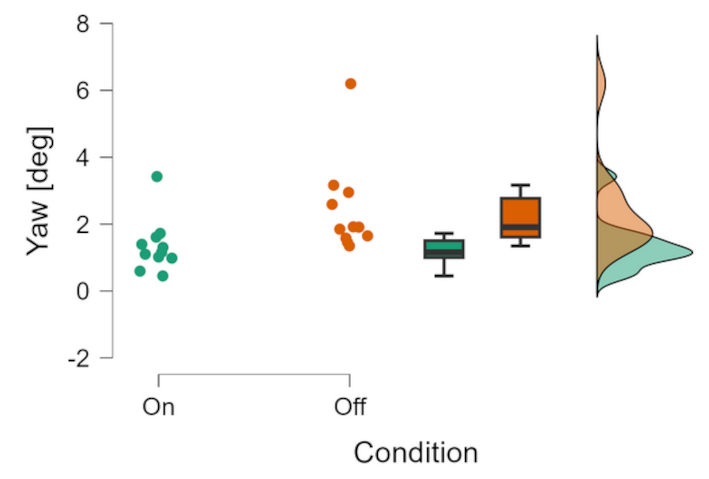
\includegraphics[width=60mm]{kickplate-results.png}}
    \caption{Representative results from each experiment.}
    \label{fig:results}
  \end{center}
\end{figure}

\section{CONCLUSIONS}
%
The balance assist system, driven by roll rate feedback steering control,
stabilizes the riderless bicycle at speeds greater than approximately
4~\si{\kph}, which is much lower than the uncontrolled minimum stable speed
of about 18~\si{\kph}. The bicycle is rideable and we show that motions resulting
from disturbances and distractions are reduced with the system on. We also show
that the probability of falling is significantly reduced at low speeds when the
system is on. Given that large steer and roll motions correlate to reduced
rider control authority and that many single actor falls occur at low
speeds~\cite{Wegman2024}, we project that wide use of a balance assisted
bicycle may reduce falls and thus injuries.

\bibliographystyle{plain}
\bibliography{references}

\end{document}
